\documentclass{boi2014-et}

\renewcommand{\DayNum}{2}
\renewcommand{\TaskCode}{demarcation}
\renewcommand{\TaskName}{Demarcation}

\newcommand{\constant}[1]{{\tt #1}}

\begin{document}

    \begin{wrapfigure}{r}{3cm}
        \vspace{-24pt}
        \includegraphics[width=3cm]{\TaskCode.jpeg}
    \end{wrapfigure}

    Kaua aega valitses Bytopia saart hea kuningas Byteasar.
    Pärast kuninga ootamatut surma ei suutnud tema kaksikud pojad
    Biteon ja Byteon otsustada, kumb neist peaks troonile asuma.
    Seetõttu otsustati saar kaheks jagada ja neid sõltumatult valitseda.

    Kaardil on Byteotia $N$ tipuga hulknurga kujuline.
    Hulknurga kõik küljed on paralleelsed ristkülikukujulise kaardi külgedega ning
    kõik järjestikused küljed paiknevad teineteise suhtes täisnurga all.
    Biteon ja Byteon tahavad hulknurga jagada kaheks kongruentseks kujundiks,
    kasutades poolitamiseks üht sirglõiku,
    mis on hulknurga sees ning paralleelne ühega kaardi külgedest.
    (Kaks kujundit on kongruentsed, kui üht saab muuta teiseks,
    kasutades peegeldusi, pööramisi ja nihutamisi.)
    Hulknurga tippude koordinaadid ja jagamiseks
    kasutatava sirglõigu otspunktide koordinaadid on täisarvud.

    Kuningapojad küsivad, kas selline jagamine on võimalik.

    \Task

    Leida saare kuju põhjal, kas seda saab horisontaalse või vertikaalse sirglõiguga
    kaheks kongruentseks kujundiks jagada.
    Kui saab, siis leida selline lõik.

    \Input

    Sisendi esimesel real on tippude arv $N$.
    Järgmisel $N$ real on igaühel tühikuga eraldatud täisarvude paar
    $X_i$ ja $Y_i$, $i$. tipu koordinaadid.
    Tipud on antud järjekorras, s.t lõigud $(X_1,Y_1) - (X_2,Y_2)$,
    $(X_2,Y_2) - (X_3,Y_3)$, \ldots, $(X_{N-1},Y_{N-1}) - (X_N,Y_N)$ ja
    $(X_N,Y_N) - (X_1,Y_1)$ on parajasti hulknurga külgedeks.

    \Output

    Programm peab väljastama ühe rea.
    Kui saare jagamine on võimalik, väljastada 4 tühikutega eraldatud täisarvu
    $x_1$, $y_1$, $x_2$ ja $y_2$, mis tähistavad sirglõiku otspunktidega
    $(x_1, y_1)$ ja $(x_2, y_2)$.
    Peab kehtima kas $x_1 = y_1$ või $y_1 = y_2$.

    Kui selline jagamine pole võimalik, väljastada sõna
    ``\constant{Impossible}'' (ilma jutumärkideta).

    \Examples
    \example
    {
        10 \newline
        0 0 \newline
        1 0 \newline
        1 1 \newline
        3 1 \newline
        3 5 \newline
        2 5 \newline
        2 3 \newline
        1 3 \newline
        1 2 \newline
        0 2
    }
    {
        1 2 3 2
    }
    {
        Selles näites on mitu võimalikku õiget vastust.

        \begin{center}
            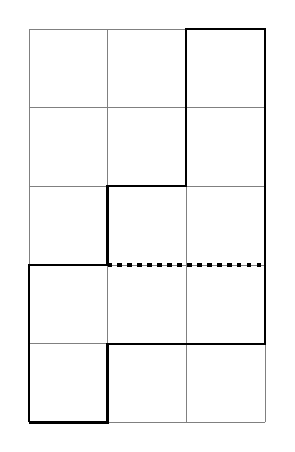
\begin{tikzpicture}
            \draw[help lines] (0,0) grid (3,5);
            \draw[thick] (0,0) -- (1,0) -- (1,1) -- (3,1) -- (3,5) --
                         (2,5) -- (2,3) -- (1,3) -- (1,2) -- (0,2) -- (0,0);
            \draw[ultra thick,dotted] (1,2) -- (3,2);
            \end{tikzpicture}
        \end{center}
    }

    \example
    {
        6 \newline
        0 0 \newline
        1 0 \newline
        1 1 \newline
        2 1 \newline
        2 2 \newline
        0 2
    }
    {
        NO
    }
    {
        Selles näites ei saa saart jagada.
        \begin{center}
            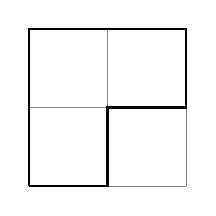
\begin{tikzpicture}
            \draw[help lines] (0,0) grid (2,2);
            \draw[thick] (0,0) -- (1,0) -- (1,1) --
                         (2,1) -- (2,2) -- (0,2) -- (0,0);
            \end{tikzpicture}
        \end{center}
    }

    \Scoring

    \begin{description}
        \item[Alamülesanne 1 (? punkti).] $4 \le N \le 200$.
        \item[Alamülesanne 2 (? punkti).] $4 \le N \le 4 000$.
        \item[Alamülesanne 3 (? punkti).] $4 \le N \le 100 000$.
    \end{description}

    \Constraints

    \begin{description}
        \item[Ajapiirang:] ? s.
        \item[Mälupiirang:] ? MB.
    \end{description}

\end{document}
